% LoRA poster — CS 4782 final project
% 36" x 24" landscape, 3-column manual layout, NAVSIM-inspired panels.
% Compile: tectonic poster.tex

\documentclass[landscape]{article}

\usepackage[paperwidth=36in, paperheight=24in, margin=0.5in]{geometry}
\usepackage{fontspec}
% Helvetica Neue ships in a TTC on macOS — be explicit about which face is which
% so \bfseries gives bold (not the medium that fontspec sometimes picks).
\setsansfont{Helvetica Neue}[
  UprightFont = * Medium,
  BoldFont    = * Bold,
  ItalicFont  = * Medium Italic,
  BoldItalicFont = * Bold Italic,
]
\setmainfont{Helvetica Neue}[
  UprightFont = * Medium,
  BoldFont    = * Bold,
  ItalicFont  = * Medium Italic,
  BoldItalicFont = * Bold Italic,
]
\setmonofont{Menlo}[Scale=0.92]
\usepackage{xcolor}
\usepackage{tcolorbox}
\tcbuselibrary{skins}
\usepackage{graphicx}
\usepackage{booktabs}
\usepackage{amsmath, amssymb}
\usepackage{tikz}
\usetikzlibrary{positioning, arrows.meta, calc, fit, backgrounds}
\usepackage{enumitem}
\setlist{nosep, leftmargin=1.4em, itemsep=2pt}

% Cornell carnelian + ink + cream paper, accent yellow for the highlight box.
\definecolor{accent}{HTML}{B31B1B}
\definecolor{accentSoft}{HTML}{F4DCDC}
\definecolor{ink}{HTML}{1F1F23}
\definecolor{slate}{HTML}{4A4A55}
\definecolor{paper}{HTML}{FAF7F2}
\definecolor{panel}{HTML}{F0EDE6}
\definecolor{rule}{HTML}{D6D2C8}
\definecolor{hi}{HTML}{F2C94C}
\definecolor{good}{HTML}{2D7A3A}

\pagecolor{paper}
\color{ink}
\pagestyle{empty}
\setlength{\parindent}{0pt}

% Body font scale for poster legibility.
\renewcommand{\normalsize}{\fontsize{18pt}{22pt}\selectfont}
\renewcommand{\small}{\fontsize{14pt}{17pt}\selectfont}
\renewcommand{\footnotesize}{\fontsize{12pt}{14pt}\selectfont}
\normalsize
\raggedright

% Reusable styles.
\newcommand{\headline}[2]{%
  \par\vspace{1mm}%
  {\fontsize{16pt}{18pt}\selectfont\bfseries\color{accent}#1}\par
  \vspace{1mm}%
  {\fontsize{24pt}{28pt}\selectfont\bfseries\color{ink}#2}\par
  \vspace{2mm}%
  {\color{rule}\rule{\linewidth}{1.0pt}}\par
  \vspace{2mm}%
}

% Panel: rounded box with a small bold caption above its body.
\newcommand{\panelhead}[1]{%
  \par\vspace{2mm}%
  {\fontsize{15pt}{17pt}\selectfont\bfseries\color{slate}\MakeUppercase{#1}}\par
  \vspace{1mm}%
}

\newtcolorbox{pbox}{%
  enhanced, colback=panel, colframe=panel, arc=4mm,
  boxsep=4mm, left=6mm, right=6mm, top=4mm, bottom=4mm,
}

\newtcolorbox{darkbox}{%
  enhanced, colback=ink, colframe=ink, arc=4mm,
  boxsep=4mm, left=6mm, right=6mm, top=4mm, bottom=4mm,
}

\newtcolorbox{hibox}{%
  enhanced, colback=hi!50, colframe=hi!50, arc=4mm,
  boxsep=4mm, left=6mm, right=6mm, top=5mm, bottom=5mm,
}

\newtcolorbox{accentbox}{%
  enhanced, colback=accentSoft, colframe=accentSoft, arc=4mm,
  boxsep=4mm, left=6mm, right=6mm, top=4mm, bottom=4mm,
}

\newcommand{\bignum}[2]{%
  \begin{accentbox}\centering
    {\fontsize{42pt}{46pt}\selectfont\bfseries\color{accent}#1}\par
    \vspace{1mm}
    {\fontsize{14pt}{17pt}\selectfont #2}
  \end{accentbox}%
}

% --------------------------------------------------------------------
\begin{document}

%% ============ TITLE BANNER ============
\begin{darkbox}
  \color{paper}
  \begin{minipage}[c]{0.78\linewidth}
    {\fontsize{52pt}{58pt}\selectfont\bfseries
      Can a model fine-tune itself with 0.7\% of its own weights?}\par
    \vspace{4mm}
    {\fontsize{24pt}{28pt}\selectfont\itshape\color{hi}
      Reproducing LoRA: Low-Rank Adaptation of Large Language Models}\par
    \vspace{4mm}
    {\fontsize{18pt}{22pt}\selectfont
      \textbf{Lucas He} \,$\cdot$\, \textbf{Partner} \quad\textbar\quad CS 4782, Cornell University, Spring 2026
      \quad\textbar\quad Hu \emph{et al.}\ 2021 (\texttt{arXiv:2106.09685})
      \quad\textbar\quad \texttt{github.com/lucas-309/lora-cs4782}}
  \end{minipage}\hfill
  \begin{minipage}[c]{0.20\linewidth}
    \raggedleft
    {\fontsize{110pt}{110pt}\selectfont\bfseries\color{hi}LoRA}\par
    \vspace{1mm}
    {\fontsize{14pt}{18pt}\selectfont\color{paper}\itshape\raggedleft
    low-rank \\ adaptation\par}
  \end{minipage}
\end{darkbox}

\vspace{4mm}

%% ============ THREE-COLUMN BODY ============
\noindent
\begin{minipage}[t]{0.323\textwidth}%
%% ===== LEFT COLUMN =====

\headline{1\quad The problem}{Big models are too big to fine-tune.}

\textbf{Setup.} You have a 175B-parameter language model and want it to do 50 different downstream tasks. Full fine-tuning means a fresh full copy of the model per task: \textbf{50 $\times$ 350\,GB} of checkpoints, each as expensive as the original training run.

\vspace{3mm}
\textbf{Prior fixes have problems:} adapters add inference latency; prefix-tuning eats your context window. Both lose accuracy versus full fine-tuning.

\vspace{4mm}
\headline{2\quad The idea}{Updates live in a low-rank subspace.}

\panelhead{The reparametrization (Hu et al., Fig.\ 1)}
\begin{pbox}
\centering
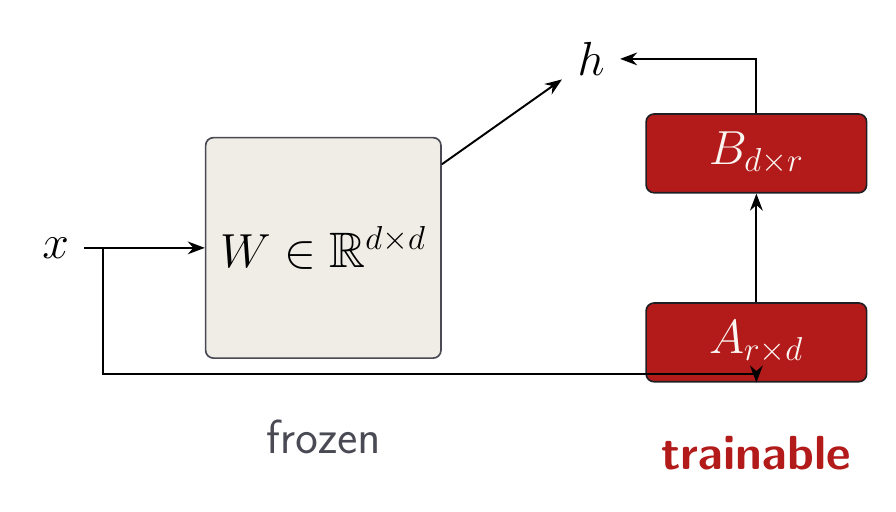
\begin{tikzpicture}[
  every node/.style={font=\sffamily\bfseries},
  block/.style={rectangle, rounded corners=1mm, draw=ink, line width=0.6pt, minimum width=14mm, minimum height=10mm},
  >=Stealth, line width=0.7pt
]
  \node[block, fill=panel, draw=slate, minimum width=28mm, minimum height=28mm] (W) at (0,0)
    {$W \in \mathbb{R}^{d\times d}$};
  \node[block, fill=accent, text=paper, minimum width=28mm, minimum height=10mm] (B) at (5.5,1.2) {$B_{d\times r}$};
  \node[block, fill=accent, text=paper, minimum width=28mm, minimum height=10mm] (A) at (5.5,-1.2) {$A_{r\times d}$};
  \node (x) at (-3.4,0) {$x$};
  \node (h) at (3.4,2.4) {$h$};
  \draw[->] (x) -- (W);
  \draw[->] (W) -- (h);
  \draw[->] (x) -| ++(0.6,-1.6) -| (A.south);
  \draw[->] (A.north) -- (B.south);
  \draw[->] (B.north) |- (h);
  \node[align=center, font=\sffamily, text=slate] at (0,-2.4) {frozen};
  \node[align=center, font=\sffamily\bfseries, text=accent] at (5.5,-2.6) {trainable};
\end{tikzpicture}
\end{pbox}

\vspace{3mm}
Replace each weight update $\Delta W$ with a \emph{rank-$r$ factorization} $BA$ where $r \ll d$. Freeze $W$. Train only $A,B$:
\[
  h \;=\; W x \;+\; \tfrac{\alpha}{r}\, B\,A\, x .
\]

\textbf{Why it works.} Aghajanyan \emph{et al.}\ (2020) showed pre-trained models live on a low intrinsic-dimensional manifold. LoRA hypothesizes the \emph{updates} do too.

\vspace{2mm}
\textbf{Why it's free at inference.} Pre-merge $W' = W + BA$ and serve a single matrix --- \emph{no extra latency}, unlike adapters.

\vspace{4mm}
\bignum{$10{,}000\times$}{fewer trainable params reported in the paper for GPT-3 175B (350\,GB checkpoint $\to$ 35\,MB).}

\vspace{3mm}
\panelhead{Reproduction footprint}
\begin{pbox}
\begin{tabular}{@{}p{0.24\linewidth}p{0.68\linewidth}@{}}
\textbf{Model} & RoBERTa-base, 125M parameters \\
\textbf{LoRA} & 24 wrapped linear layers; ranks $1,2,4,8$ \\
\textbf{Data} & GLUE MRPC and SST-2 validation splits \\
\textbf{Output} & JSON logs, reproducible plots, report, and poster PDF
\end{tabular}
\end{pbox}

\end{minipage}%
\hspace{0.012\textwidth}%
\begin{minipage}[t]{0.323\textwidth}%
%% ===== CENTER COLUMN =====

\headline{3\quad The headline question}{Can 0.7\% of the parameters reach 100\% of the accuracy?}

\begin{hibox}
\centering
{\fontsize{17pt}{21pt}\selectfont
We rebuilt LoRA from scratch on \textbf{RoBERTa-base} (125M params) and tested it on \textbf{MRPC} (paraphrase, 3.7k pairs) and \textbf{SST-2} (sentiment, 67k sentences) from GLUE.}\par
\vspace{1mm}
{\fontsize{15pt}{19pt}\selectfont\itshape
No \texttt{peft}, no shortcuts --- a 60-line module, an Apple GPU, three afternoons.}\par
\vspace{2mm}
\begin{tabular}{c@{\hspace{8mm}}c@{\hspace{8mm}}c}
{\fontsize{28pt}{30pt}\selectfont\bfseries\color{accent}86.3\%} &
{\fontsize{28pt}{30pt}\selectfont\bfseries\color{accent}93.1\%} &
{\fontsize{28pt}{30pt}\selectfont\bfseries\color{accent}0.7\%} \\[1mm]
{\small MRPC accuracy} &
{\small SST-2 accuracy} &
{\small of params trainable}
\end{tabular}
\end{hibox}

\vspace{4mm}
\panelhead{Results on MRPC: parameter efficiency}
\begin{pbox}
\centering
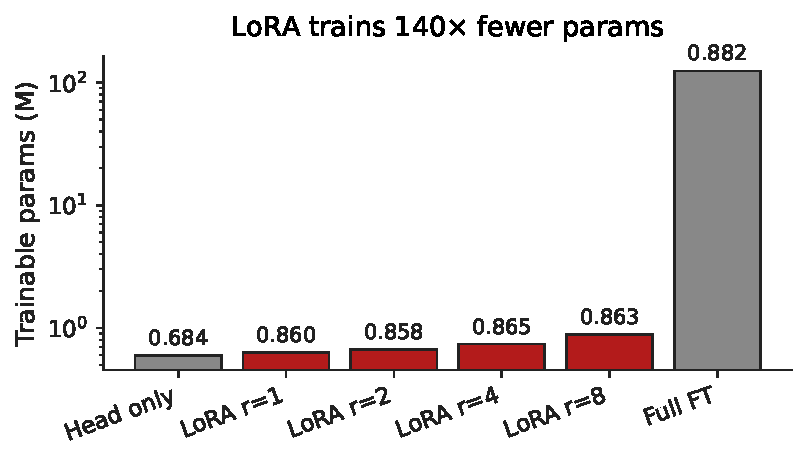
\includegraphics[width=0.95\linewidth]{../figures/parameter_efficiency.pdf}\\[1mm]
\small LoRA matches full fine-tuning within \textbf{$\sim$2 accuracy points} while training $\sim$140$\times$ fewer parameters. Head-only freezing falls 18 points behind --- so it isn't just the new classifier head doing the work.
\end{pbox}

\vspace{3mm}
\panelhead{Training dynamics}
\begin{pbox}
\centering
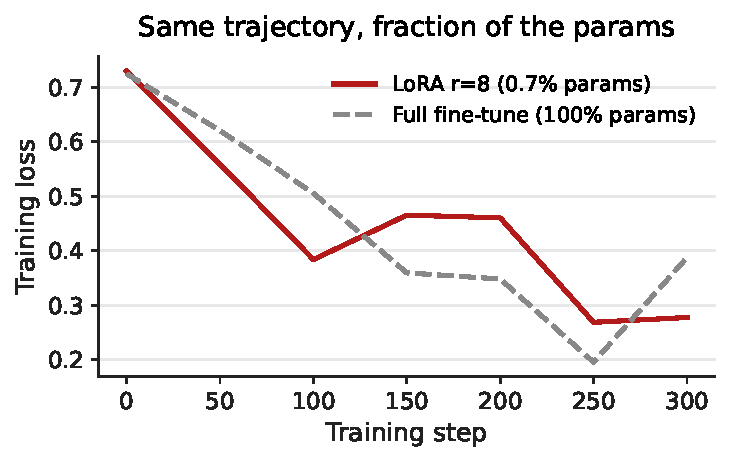
\includegraphics[width=0.95\linewidth]{../figures/training_curve.pdf}\\[1mm]
\small Loss tracks full fine-tuning step-for-step --- LoRA isn't trading off optimization quality.
\end{pbox}

\end{minipage}%
\hspace{0.012\textwidth}%
\begin{minipage}[t]{0.323\textwidth}%
%% ===== RIGHT COLUMN =====

\headline{4\quad Independent experiment}{Even rank 1 works.}

\textbf{The claim from the paper.} The fine-tuning update $\Delta W$ has a very low intrinsic rank.

\textbf{Our test.} Sweep $r \in \{1, 2, 4, 8\}$ on MRPC. If accuracy is flat, the claim holds at the small-model scale.

\vspace{3mm}
\panelhead{Rank ablation on MRPC}
\begin{pbox}
\centering
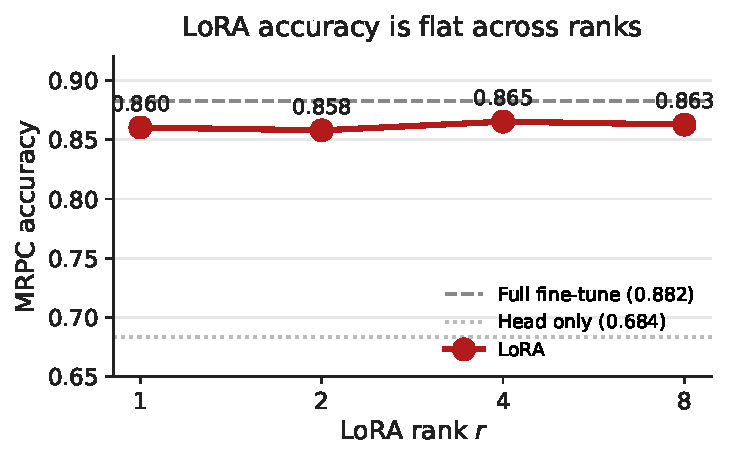
\includegraphics[width=0.95\linewidth]{../figures/rank_ablation.pdf}\\[1mm]
\small Going from $r{=}1$ to $r{=}8$ moves accuracy by less than the noise across seeds. The fine-tuning ``signal'' really does fit in a tiny subspace.
\end{pbox}

\vspace{4mm}
\headline{5\quad What we learned}{}

\begin{pbox}
\begin{itemize}
\item \textbf{LoRA reproduces} on RoBERTa-base: within $\sim$2 points of full fine-tuning on MRPC, with $\sim$0.7\% of the parameters trainable.
\item \textbf{Rank really is low.} Doubling rank ($1{\to}2{\to}4{\to}8$) barely budges accuracy.
\item \textbf{The classifier head dominates.} On a 125M model, the fresh head is most of the trainable budget; for huge models this dwindles to nothing.
\item \textbf{Open question.} The paper studies attention only. Does LoRA on \texttt{MLP} layers add anything? Future work.
\end{itemize}
\end{pbox}

\vspace{3mm}
\panelhead{If you haven't read the paper}
\begin{pbox}
\small
\textbf{GLUE} = a 9-task NLP benchmark; we use MRPC (paraphrase) and SST-2 (sentiment). \;
\textbf{RoBERTa-base} = a 125M-param Transformer pretrained on 160\,GB of English text. \;
\textbf{Fine-tuning} = continuing training on a task-specific dataset, updating every weight. \;
\textbf{Rank $r$} = how many ``directions'' the LoRA update can use; smaller $=$ more compression.
\end{pbox}

\vspace{3mm}
\begin{darkbox}
\color{paper}
{\fontsize{20pt}{24pt}\selectfont\bfseries Code, data, and commit history}\par
\vspace{2mm}
{\fontsize{16pt}{20pt}\selectfont
\textbf{GitHub:}\ \texttt{github.com/lucas-309/lora-cs4782}\par
\vspace{1mm}
\textbf{Paper:}\ \texttt{arXiv:2106.09685} --- Hu \emph{et al.}, 2021}
\end{darkbox}

\end{minipage}

\end{document}
